% Options for packages loaded elsewhere
\PassOptionsToPackage{unicode}{hyperref}
\PassOptionsToPackage{hyphens}{url}
%
\documentclass[
]{article}
\usepackage{amsmath,amssymb}
\usepackage{lmodern}
\usepackage{iftex}
\ifPDFTeX
  \usepackage[T1]{fontenc}
  \usepackage[utf8]{inputenc}
  \usepackage{textcomp} % provide euro and other symbols
\else % if luatex or xetex
  \usepackage{unicode-math}
  \defaultfontfeatures{Scale=MatchLowercase}
  \defaultfontfeatures[\rmfamily]{Ligatures=TeX,Scale=1}
\fi
% Use upquote if available, for straight quotes in verbatim environments
\IfFileExists{upquote.sty}{\usepackage{upquote}}{}
\IfFileExists{microtype.sty}{% use microtype if available
  \usepackage[]{microtype}
  \UseMicrotypeSet[protrusion]{basicmath} % disable protrusion for tt fonts
}{}
\makeatletter
\@ifundefined{KOMAClassName}{% if non-KOMA class
  \IfFileExists{parskip.sty}{%
    \usepackage{parskip}
  }{% else
    \setlength{\parindent}{0pt}
    \setlength{\parskip}{6pt plus 2pt minus 1pt}}
}{% if KOMA class
  \KOMAoptions{parskip=half}}
\makeatother
\usepackage{xcolor}
\IfFileExists{xurl.sty}{\usepackage{xurl}}{} % add URL line breaks if available
\IfFileExists{bookmark.sty}{\usepackage{bookmark}}{\usepackage{hyperref}}
\hypersetup{
  pdftitle={Different rules for binocular combination of luminance in cortical and subcortical pathways},
  pdfauthor={Federico G. Segala, Aurelio Bruno, Alex R. Wade \& Daniel H. Baker (+Myat? +Joel?)},
  hidelinks,
  pdfcreator={LaTeX via pandoc}}
\urlstyle{same} % disable monospaced font for URLs
\usepackage[margin=1in]{geometry}
\usepackage{longtable,booktabs,array}
\usepackage{calc} % for calculating minipage widths
% Correct order of tables after \paragraph or \subparagraph
\usepackage{etoolbox}
\makeatletter
\patchcmd\longtable{\par}{\if@noskipsec\mbox{}\fi\par}{}{}
\makeatother
% Allow footnotes in longtable head/foot
\IfFileExists{footnotehyper.sty}{\usepackage{footnotehyper}}{\usepackage{footnote}}
\makesavenoteenv{longtable}
\usepackage{graphicx}
\makeatletter
\def\maxwidth{\ifdim\Gin@nat@width>\linewidth\linewidth\else\Gin@nat@width\fi}
\def\maxheight{\ifdim\Gin@nat@height>\textheight\textheight\else\Gin@nat@height\fi}
\makeatother
% Scale images if necessary, so that they will not overflow the page
% margins by default, and it is still possible to overwrite the defaults
% using explicit options in \includegraphics[width, height, ...]{}
\setkeys{Gin}{width=\maxwidth,height=\maxheight,keepaspectratio}
% Set default figure placement to htbp
\makeatletter
\def\fps@figure{htbp}
\makeatother
\setlength{\emergencystretch}{3em} % prevent overfull lines
\providecommand{\tightlist}{%
  \setlength{\itemsep}{0pt}\setlength{\parskip}{0pt}}
\setcounter{secnumdepth}{5}
\newlength{\cslhangindent}
\setlength{\cslhangindent}{1.5em}
\newlength{\csllabelwidth}
\setlength{\csllabelwidth}{3em}
\newlength{\cslentryspacingunit} % times entry-spacing
\setlength{\cslentryspacingunit}{\parskip}
\newenvironment{CSLReferences}[2] % #1 hanging-ident, #2 entry spacing
 {% don't indent paragraphs
  \setlength{\parindent}{0pt}
  % turn on hanging indent if param 1 is 1
  \ifodd #1
  \let\oldpar\par
  \def\par{\hangindent=\cslhangindent\oldpar}
  \fi
  % set entry spacing
  \setlength{\parskip}{#2\cslentryspacingunit}
 }%
 {}
\usepackage{calc}
\newcommand{\CSLBlock}[1]{#1\hfill\break}
\newcommand{\CSLLeftMargin}[1]{\parbox[t]{\csllabelwidth}{#1}}
\newcommand{\CSLRightInline}[1]{\parbox[t]{\linewidth - \csllabelwidth}{#1}\break}
\newcommand{\CSLIndent}[1]{\hspace{\cslhangindent}#1}
\ifLuaTeX
  \usepackage{selnolig}  % disable illegal ligatures
\fi

\title{Different rules for binocular combination of luminance in cortical and subcortical pathways}
\author{Federico G. Segala, Aurelio Bruno, Alex R. Wade \& Daniel H. Baker (+Myat? +Joel?)}
\date{2022-10-04}

\begin{document}
\maketitle

\hypertarget{abstract}{%
\section{Abstract}\label{abstract}}

\hypertarget{introduction}{%
\section{Introduction}\label{introduction}}

Binocular combination provides a higher visual sensitivity than monocular viewing. This superiority is known as binocular summation and is defined by the binocular summation ratio (BSR), which was originally believed to be around \(\sqrt{2}\) (\(\approx1.4\)) for grating stimuli at detection threshold (Campbell and Green, 1965). In other words, a monocular stimulus can elicit the same response as a binocular stimulus if it has a contrast that is 1.4 times higher. This led Legge to develop a widely accepted explanation that used quadratic summation to describe binocular combination (Legge, 1984): monocular signals from the right (R) and the left (L) eyes are squared before being summed together and the binocular response (B) is given by the square root of the output (B = \(\sqrt{R^2 + L^2}\), when R and L are equal to 1, the output is \(\sqrt{2}\)). However, subsequent research has shown that these explanations are not fully adequate to account for binocular summation. Both of these accounts constitute single channel models, and this type of model has been shown to not being able to account for contrast detection in the presence of noise (Anderson and Movshon, 1989). Moreover, more recent research has shown that the summation ratio can vary greatly between \(\sqrt{2}\) and 2 depending on factors such as the spatial and temporal frequency of a stimulus or the sensitivity difference between the eyes (Baker et al., 2018). These observations led to the development of multistage gain control models, which combine binocular summation and interocular suppression, and can account for contrast matching, detection and discrimination for spatial contrast (Ding and Sperling, 2006; Meese et al., 2006).

In general, it seems that the mechanisms behind binocular combination have been thoroughly studied, as have been the anatomical pathways behind it: light enters the eye though the pupil and signals are sent from the left and right retinae to the primary visual cortex, remaining anatomically isolated while passing through the lateral geniculate nucleus (LGN) until they reach V1, where they are binocularly combined (Purves et al., 2008). However, there is an eye component that is often underestimated in its role to determine the quality of visual information: the pupil. The pupils are openings found in the centre of the eyes that appear to be black and allow light to enter the eyes. Their size determines how much light will reach the retina and it is usually determined by the ambient levels of light: in brightness the pupils will constrict and in darkness they will dilate. This is known as the pupillary light response (PLR). The anatomical pathways that regulate this response are well understood and are very clearly and extensively described in the literature (Angée et al., 2021; Mathôt, 2018; McDougal and Gamlin, 2010; Wang and Munoz, 2015). However, they are anatomically distinct from the LGN-V1 pathway meaning that binocular combination occurs separately in anatomically distinct pathways. Given this, not much is known about the computational processes behind the PLR except for some evidence of binocular interaction. The presence of a consensual response in one eye when the other is being stimulated, and the presence of convergence (one pupil responds to illumination in either retina) and divergence (both pupils respond to illumination of one retina) (Wyatt and Musselman, 1981) are evidence of this binocular interaction.

With this in mind we designed an experiment that simultaneously recorded electrophysiological and pupillometric responses to investigate the combination of flickering light signals in both the visual cortex and the pupils. The results should offer new insight about basic neural circuits and information on how they might be affected in clinical disorders of vision (e.g.~amblyopia). Based on previous literature, we expected to find a non-linear combination of the responses in visual cortex, as described by the gain control mechanisms, and a more linear combination of the responses and a greater binocular response at the level of the pupils.

To follow up on the results that we obtained, we decided to perform a contrast matching experiment to investigate whether perception of flickering light is consistent with the results observed in the cortical pathways (visual cortex) or the subcortical pathways (pupils). Matching is a paradigm in which the perceived brightness of a standard stimulus is matched to that of a target stimulus. In the latter, the interocular ratios of luminance are varied to obtain an equibrightness curve. Previous literature has used this paradigm to investigate the binocular fusion of static stimuli and the temporal combination of spatial flickering of spatial increments (a bright target on a dark background) and decrements (a dark target on a bright background) (Anstis and Ho, 1998; Levelt, 1965). For spatial increments, it was found that binocular fusion seems to follow approximately linear combination rules. This means that, for a monocular stimulus to elicit the same response as a binocular stimulus, the former needs to have twice the signal of the latter. On the other hand, spatial decrements follow a winner-takes-all pattern. This means that the observer is seeing what the eye that is receiving the strongest signal is seeing.

Our experiment used different stimuli than the ones used by Anstis and Ho: in the binocular fusion experiment, their stimuli were not flickering and, in the flicker experiment, they were always shown in both eyes. In our experiment, in some conditions, the flicker was shown to only one eye. Moreover, they were looking at the temporal fusion of the flicker while we focussed on the binocular fusion of the flicker. Based on this and on the results from our first experiment, we expected to find a near linear summation of the responses.

\hypertarget{methods}{%
\section{Methods}\label{methods}}

\hypertarget{participants}{%
\subsection{Participants}\label{participants}}

Thirty, twelve and ten participants were recruited for experiment 1, 2 and 3 respectively. All participants had normal or corrected to normal binocular vision. All participants gave written informed consent.

\hypertarget{apparatus-stimuli}{%
\subsection{Apparatus \& Stimuli}\label{apparatus-stimuli}}

The stimuli were two discs of flickering light with a diameter of 3.74 degrees, presented on a black background. The same stimuli were used for all three experiments. Four dark red lines were added around both discs to help with their fusion into one binocular disc (see insert in figure \ref{fig:pupildata}a for an example of the of the fused stimuli). The discs were viewed through a four-mirror stereoscope, which used front silvered mirrors and so did not suffer from internal reflections, and allowed participants to see only one fused disc. The use of a stereoscope allowed us to display the stimuli in three different ocular configurations: monocular, binocular, and dichoptic.

All stimuli were displayed at a mean luminance of 42 cd/m\(^2\) on an Iiyama Vision Master™ Pro 510 display (800 x 600 pixels, 60 Hz refresh rate), which was gamma corrected using a Minolta LS-110 (Minolta Camera Co.~Ltd., Japan). For experiments 1 and 2, the stimuli were presented using Psychopy (v3.0.7). For experiment 3, the stimuli were presented using Psychopy (v2022.1.1).

EEG data were collected for experiments 1 and 2 sampled at 1 kHz using a 64-electrode ANT WaveGuard cap and the signals were recorded using the ASA software (ANT Neuro, Hengelo, NL, United States). Pupillometry data were collected only for experiment 1 using a binocular Pupil Core eye-tracker (Pupil Labs GmbH, Kassner et al. (2014)) running at 120 Hz and the signals were recorded with the Pupil Capture software (Pupil Labs GmbH, Kassner et al. (2014)).

\hypertarget{procedure}{%
\subsection{Procedure}\label{procedure}}

Before each experiment, participants calibrated the stereoscope by adjusting the angle of the mirrors. This was done so that they would perceive the two discs as one fused disc when looking at the screen through the stereoscope.

\hypertarget{experiment-1}{%
\subsubsection{Experiment 1}\label{experiment-1}}

The experiment was conducted in a windowless room, in which the only light source was the monitor. The participants sat at 99 cm from the monitor and their viewing distance through the stereoscope was 107 cm. The experiment was carried out in one session lasting 45 minutes in total, divided in three blocks of 15 minutes each. In each block, there were 60 trials in total lasting 15 seconds each (12s of stimulus presentation, with an interstimulus interval of 3s). The participants had no task and were asked to look at the fixation crosses in the middle of the two discs while trying to minimise their blinking during the presentation period. The discs flickered in counterphase at 2 Hz, but in some conditions (cross-frequency conditions) one of the two discs flickered at 1.6 Hz. They were set at five temporal contrast levels relative to the mean luminance: 6, 12, 24, 48 and 96 \%.

As already stated, the mirror stereoscope allowed the use of three different ocular configurations. In the monocular configuration, one disc was set to flicker either at 2 Hz or 1.6 Hz for each contrast level, while the other disc remained stable at a constant mean luminance. In the binocular configuration, both discs flickered at the same contrast level with both discs flickering at 2 Hz in the same-frequency condition, while, in the cross-frequency condition, one disc flickered at 2 Hz and the other at 1.6 Hz. Finally, in the dichoptic configuration, one disc flickered across all contrast levels and the other flickered at a fixed contrast level that was set at 48 \%. Similar to the binocular configuration, the dichoptic configuration was divided in same-frequency and cross-frequency conditions.

\hypertarget{experiment-2}{%
\subsubsection{Experiment 2}\label{experiment-2}}

The conditions were similar to experiment 1 (windowless room and viewing distance of 107 cm). Like in experiment 1, participants had no specific task other than looking at the fixation crosses and minimising their blinking. Unlike the first experiment, only one contrast level was used (96 \%) and the discs were set to flicker at five different frequencies (2, 4, 8, 16 and 30 Hz). Only two ocular configurations, monocular and binocular, were used, with the latter having both discs flickering at the same frequency.

The experiment was carried out in one session lasting 25 minutes in total, divided in five blocks of 5 minutes each. In each block, there were 20 trials in total lasting 15 seconds each (12s of stimulus presentation and 3s of interstimulus interval).

\hypertarget{experiment-3}{%
\subsubsection{Experiment 3}\label{experiment-3}}

The experiment was conducted in a room with a blacked-out window. The sitting and viewing distances of the participants were similar to the two previous experiments. As this was a psychophysical task, no EEG or pupillometry data were collected for this experiment.

A two-interval forced-choice staircase procedure was used to collect data. In one interval, participants were presented with a standard fused disc that flickered at a set contrast level (either 24 or 48 \%), which was selected by the experimenter at the beginning of each block. In a separate interval, a target fused disc flickering at varying contrast levels was displayed. The contrast level of the target was controlled by a 1-up, 1-down staircase moving in logarithmic (dB) steps of contrast. The ratio of flicker amplitudes in the left and right eyes was varied across blocks and was set to be 0, 0.25, 0.5, 0.75 or 1. The standard and the target fused discs were displayed for 1 second each, with an interstimulus interval of 0.5 seconds. After the discs appeared on screen, the participants had to indicate which interval they perceived as having the more intense flicker. The intervals were randomly ordered, and all discs flickered at a frequency of 2 Hz.

Due to its long duration (162 minutes in total), the participants completed the experiment across multiple sessions divided at their own discretion. The experiment was divided in 54 blocks (3 repetitions \(\times\) 2 standard contrasts \(\times\) 9 target ratios), which lasted on average 3 minutes each (depending on the response speed of the participant). In each block, there were a total of 50 trials. We pooled the data from all repetitions of a given condition and fitted a cumulative normal psychometric function to estimate the point of subjective equality at the 50 \% point.

\hypertarget{data-analysis}{%
\subsection{Data analysis}\label{data-analysis}}

EEG data were converted from the ANT-EEProbe format to a compressed csv text file using a custom Matlab script and components of the EEGlab toolbox (Delorme and Makeig, 2004). The data for each participant were then loaded into R for analysis where a ten-second waveform for each trial at each electrode was extracted. Fourier transform was calculated for each waveform, and the spectrum stored in a matrix. All repetitions of each condition were then averaged for each electrode. They were then averaged across the four occipital electrodes (POz, Oz, O1, O2), to obtain individual results. Finally, these were averaged across all participants to obtain the final results.

A similar process was adopted for the analysis of the pupillometry data. The data were converted from the mp4 format to a csv text file using the Pupil Player software (Kassner et al., 2014). The individual data were then loaded into R for analysis where a twelve-second waveform for each trial in each eye was extracted. Fourier transform was calculated for each waveform, and the spectrum stored in a matrix. All repetitions of each condition were then averaged for each eye. They were then averaged across the two eyes, to obtain individual results. Finally, these were averaged across all participants to obtain the final results.

\hypertarget{results}{%
\section{Results}\label{results}}

\hypertarget{experiment-1-1}{%
\subsection{Experiment 1}\label{experiment-1-1}}

The results from the first experiment are shown in figure \ref{fig:pupildata} and figure \ref{fig:EEGdata}. Each curve is showing the amplitude of the signal for the three different configurations (monocular, binocular and dichoptic).

Figure \ref{fig:pupildata} is showing the results for the pupillometry. Figure \ref{fig:pupildata}a is showing the group average waveform for binocular presentation. Figure \ref{fig:pupildata}b is showing the average Fourier spectrum, where we can observe a spike at 2 Hz, which shows a very clear, non-noisy response to the flickering stimuli. Figures \ref{fig:pupildata}c-e show the contrast response functions (CRFs) at 2 and 1.6 Hz. In the same-frequency condition at 2 Hz (fig.~\ref{fig:pupildata}c), the amplitude of the binocular configuration is bigger than the amplitude of the monocular configuration. In general, we observe that the binocular to monocular ratio is roughly \(\sqrt2\) at each contrast level (fig.~).
In the cross-frequency condtion at 2 Hz (fig.~\ref{fig:pupildata}d), no summation is observed since the amplitudes of the binocular and dichoptic conditions are smaller than the amplitude of the monocular condition. Interestingly, we observe a relatively small cross-frequency facilitation at 1.6 Hz (fig.~\ref{fig:pupildata}e), with the binocular amplitude being bigger than the monocular amplitude, especially at the lower contrast levels. This facilitation is then lost at the highest contrast level, where the amplitude of the monocular signal is equal to the amplitude of the binocular signal. This pattern of results in the cross-frequency conditions suggests the presence of interocular suppression at the level of the pupils. Moreover, the low summation observed in the same-frequency condition suggests that theprocessing of temporal luminance modulations happens in a non-linear way at the level of the pupils.

Figure \ref{fig:EEGdata} shows the results for EEG. Figure \ref{fig:EEGdata}a is showing the group average waveform for binocular presentation. Figure \ref{fig:EEGdata}b is showing the average Fourier spectrum, where we can observe two spikes at 2 and 4 Hz, which show a very clear, non-noisy response to the flickering stimuli at the first and second harmonics. Figures \ref{fig:EEGdata}c-e show the CRFs at 2 and 1.6 Hz at the first harmonic, and figures \ref{fig:EEGdata}f-h show the CRFs at the second harmonic.
What is immediately apparent is that, in the same-frequency condition, the binocular responses at the first (fig.~\ref{fig:EEGdata}c) and second (fig.~\ref{fig:EEGdata}f) harmonics are showing very high summation of binocular signals compared to the pupillometry. The amplitudes of the binocular responses are twice, and even more than twice, the amplitudes of the monocular responses. This is especially clear at the highest contrasts. This is clearly displayed in figure, which is showing the binocular to monocular ratios for the EEG at both harmonics and the pupillometry. For the cross-frequency condition at 2 Hz and 4 Hz (fig.~\ref{fig:EEGdata}d and \ref{fig:EEGdata}g), there is almost no summation, with the amplitudes of the binocular and dichoptic configurations being equal, and even smaller, than the amplitudes of the monocular signals. This pattern is also observable in the cross-frequency condition at 1.6 (fig.~\ref{fig:EEGdata}e) and 3.2 Hz (fig.~\ref{fig:EEGdata}h). This pattern of results seems to suggest that processing of temporal luminance modulations happens in a linear way in the visual cortex. Moreover, the lower amplitudes for the binocular and the dichoptic configurations in the cross-frequency conditions seem to indicate the presence of interocular suppression in the visual cortex.

\begin{figure}

{\centering 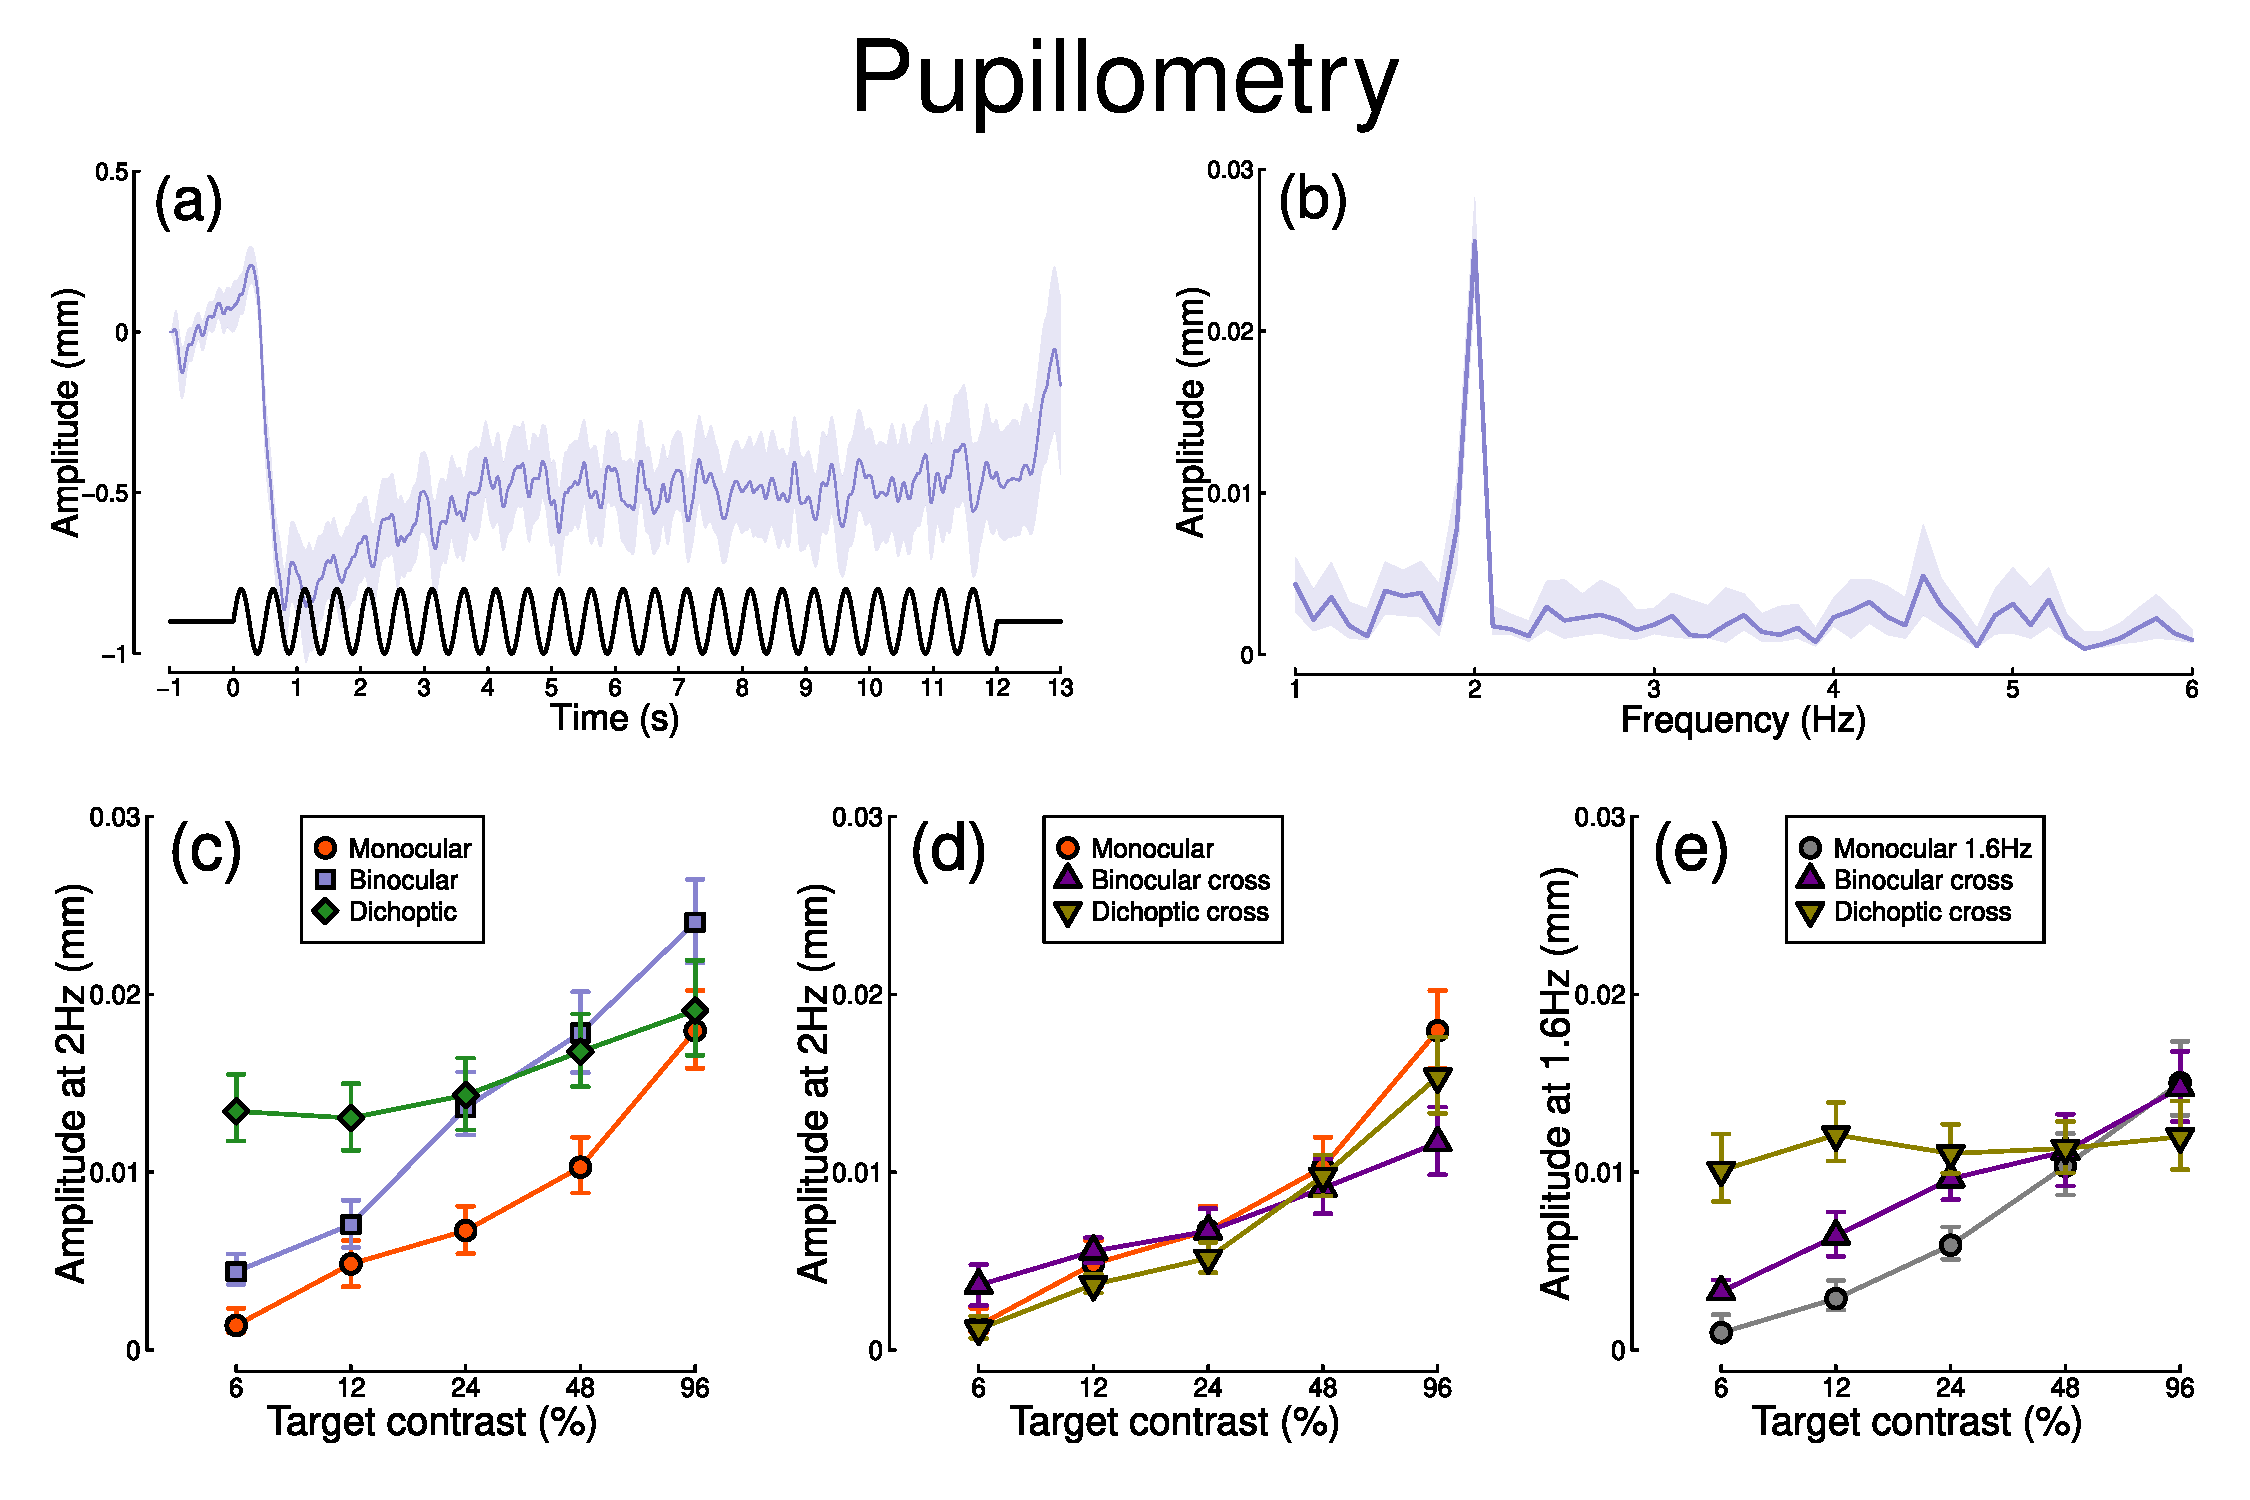
\includegraphics{Figures/pupildata} 

}

\caption{Summary of pupillometry results for N=30 participants. Panel (a) shows a group average waveform for binocular presentation (low pass filtered at 5Hz), with the driving signal plotted at the foot. Panel (b) shows the average Fourier spectrum. Panels (c,d) show contrast response functions at 2Hz for different conditions. Panel (e) shows contrast response functions at 1.6Hz for three conditions. Shaded regions and error bars indicate bootstrapped standard errors.}\label{fig:pupildata}
\end{figure}

\begin{figure}

{\centering 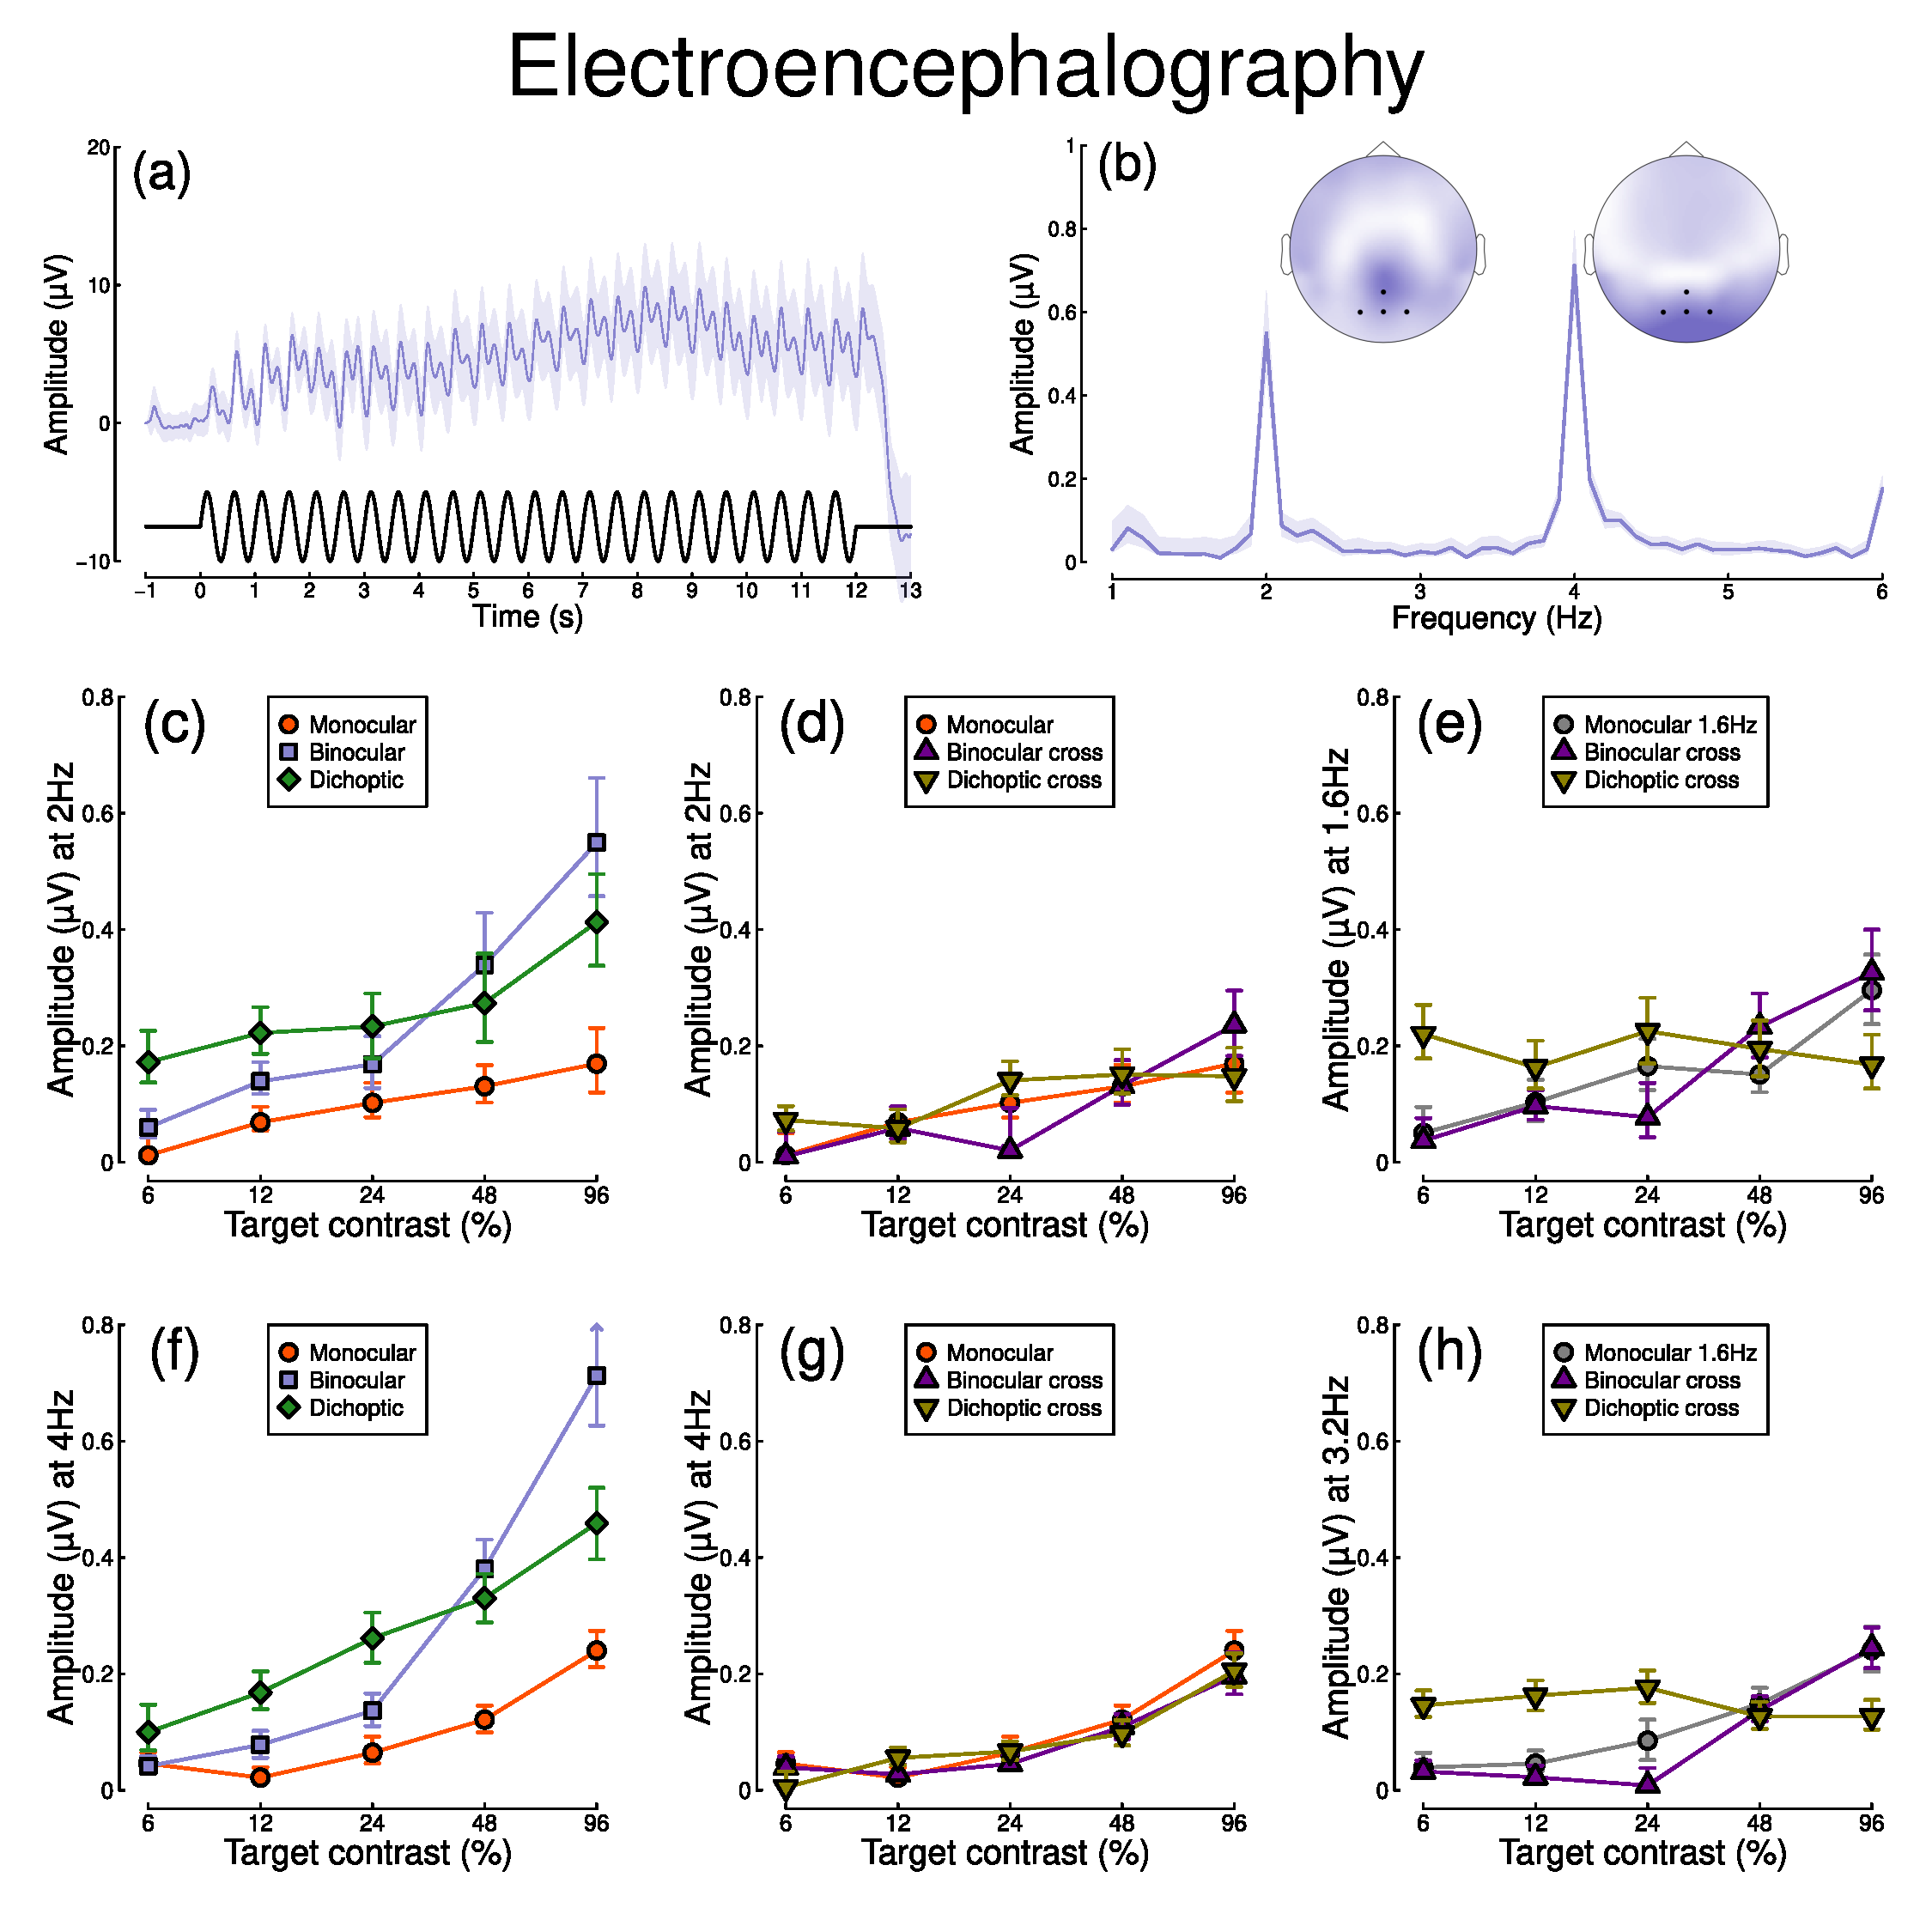
\includegraphics{Figures/EEGdata} 

}

\caption{Summary of EEG results for N=30 participants. Panel (a) shows a group average waveform for binocular presentation (low pass filtered at 5Hz), with the driving signal plotted at the foot. Panel (b) shows the average Fourier spectrum, and inset scalp distributions. Black dots on the scalp plots indicate electrodes Oz, POz, O1 and O2. Panels (c,d) show contrast response functions at 2Hz for different conditions. Panel (e) shows contrast response functions at 1.6Hz for three conditions. Panels (f-h) are in the same format but for the second harmonic responses. Shaded regions and error bars indicate bootstrapped standard errors.}\label{fig:EEGdata}
\end{figure}

\hypertarget{experiment-2-1}{%
\subsection{Experiment 2}\label{experiment-2-1}}

The results from the second experiment are shown in \ref{fig:TFdata}. Figure \ref{fig:TFdata}a is showing the Fourier spectra for responses to binocular flicker at the 5 different frequencies (2, 4, 8, 16, 30 Hz). We can observe that from 2 to 16 Hz, we recorded very clear and significant signals, as we can observe spikes at the respective frequencies and their subsequent harmonics. However, at 30 Hz, the responses recorded were mainly noise, with no clear data recorded. This is also reflected in figure \ref{fig:TFdata}b, where we observe almost no amplitude recorded for monocular and binocular responses at 30 Hz. The rest of figure \ref{fig:TFdata}b is showing the response at each stimulation frequency. We can see that there is an increase in the amplitudes from 2 Hz to 8 Hz and a decrease at 16 Hz. In general, we observe that the binocular response is twice, and more than twice, the monocular response from 2 to 16 Hz (fig.~\ref{fig:TFdata}c), suggesting that binocular facilitation is happening at higher frequencies. However, at 30 Hz, this facilitation is lost (the binocular and monocular responses are the same, as demonstrated by the binocular to monocular ratio being 1in figure \ref{fig:TFdata}c). The fact that the signal recorded at the highest frequency is mainly noise would seem to suggest that the visual cortex cannot process temporal luminance modulations anymore.

\begin{figure}

{\centering 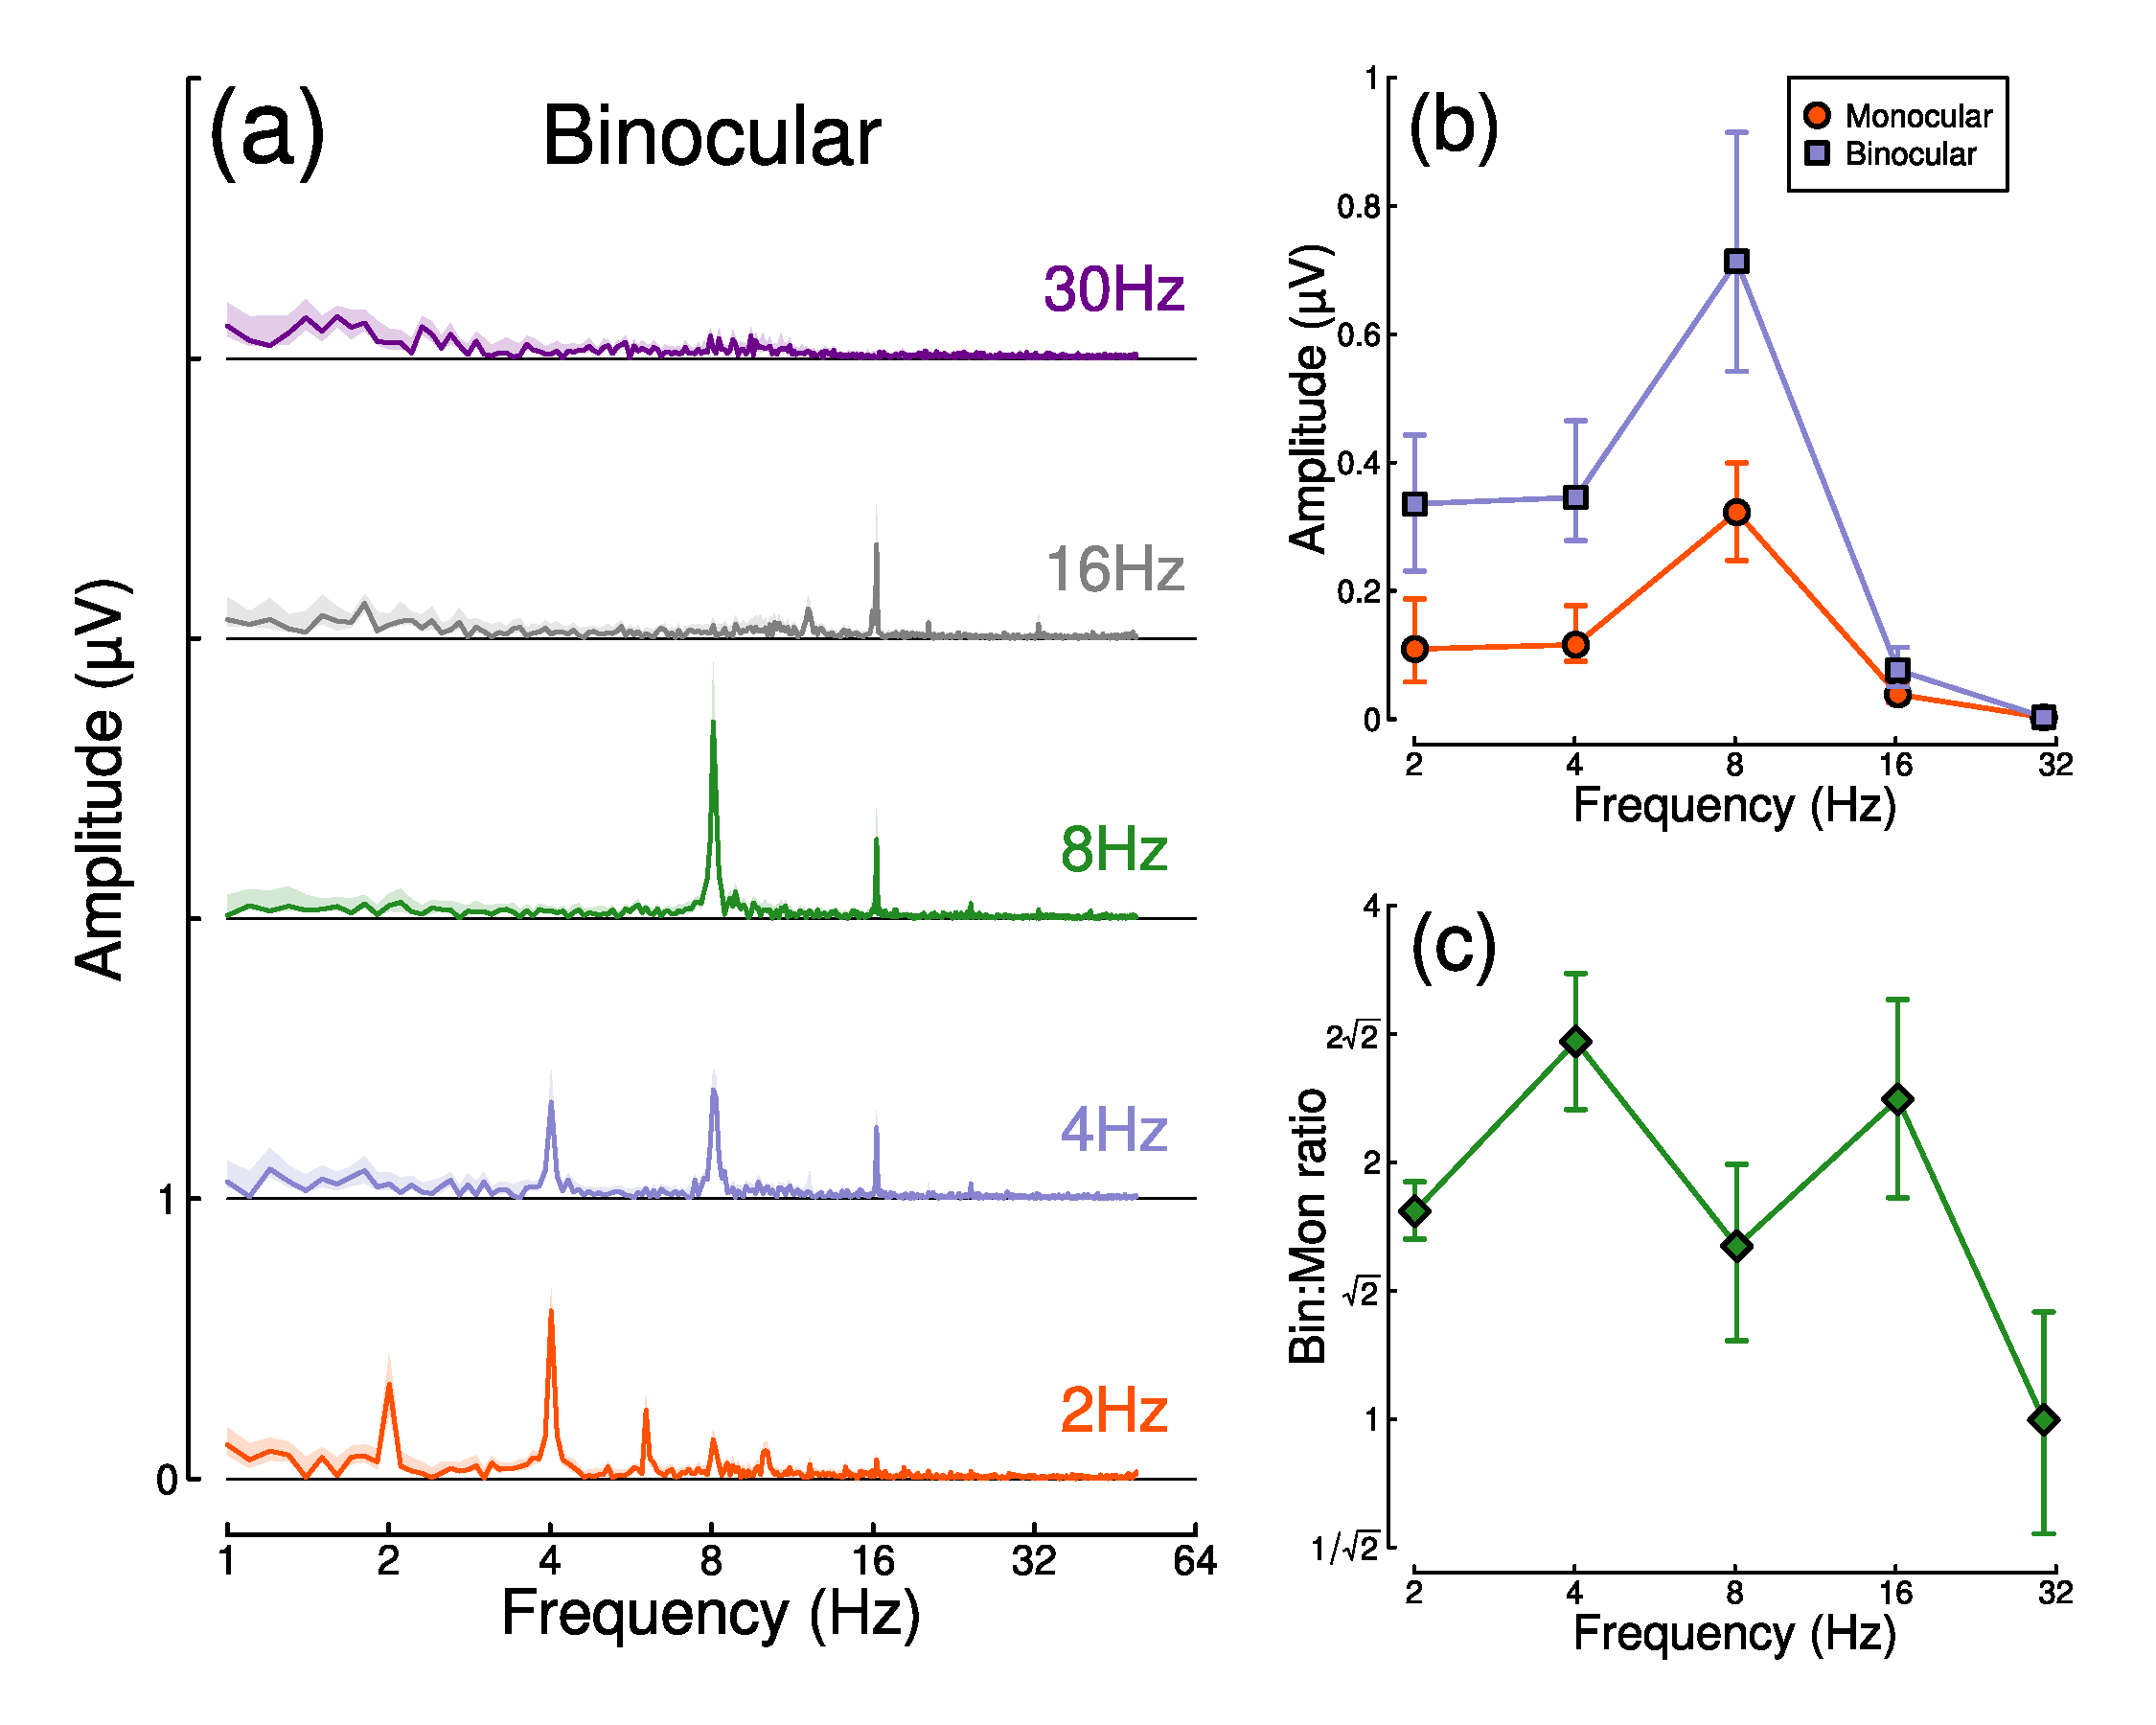
\includegraphics{Figures/TFdata} 

}

\caption{Binocular facilitation at different temporal frequencies. Panel (a) shows Fourier spectra for responses to binocular flicker at 5 different frequencies (offset vertically for clarity). Panel (b) shows the response at each stimulation frequency for monocular (red) and binocular (blue) presentation. Panel (c) shows the ratio of binocular to monocular responses. Error bars and shaded regions indicate bootstrapped standard errors across N=12 participants.}\label{fig:TFdata}
\end{figure}

\hypertarget{experiment-3-1}{%
\subsection{Experiment 3}\label{experiment-3-1}}

The results from the third experiment are shown in figure \ref{fig:matchingdata}. Each curve is showing the contrast level in each eye for the different interocular ratios at the 24 \% (in red) and 48 \% (in blue) conditions.

Looking at the results for the 48 \% contrast condition, we can observe that, when the match was presented binocularly (both eyes saw the same stimulus), the match appeared to have the same flickering intensity as the standard when the contrast in both eyes was selected to be, on average, 50 \% (red line). This is also observable for the 24 \% contrast condition, where the match appeared to have the same flickering intensity as the standard when the contrast was selected to be around 25 \%. These two results show that the paradigm was working correctly and that the participants could see the flicker properly.

When the match was presented monocularly (only one eye was presented with a flickering stimulus), we observe that, for the match to appear to flicker similarly to the standard, the contrast in that eye was set to be around double the contrast of the standard. When the flicker was presented only to the left eye, for the 48 \% contrast, the contrast of the match was around 90 \%, and, for the 24 \% contrast, the contrast of the match was around 57 \%. When the flicker was presented only to the right eye, for the 48 \% contrast, the contrast in the right eye was around 96 \%, and, for the 24 \% contrast, the contrast was around 50 \%. When looking at the intermediate condition, we can see that the points, for both contrast conditions, seem to fall along the main diagonal representing the linear summation prediction, with the results for the 24 \% condition showing a very strong summation that seem to exceed this prediction. Overall, these results seem to suggest that the way we perceive temporal luminance modulations follows near linear combination rules, which is in line with the processes observed in the visual cortex in experiment 1 (fig.~\ref{fig:EEGdata}).

\begin{figure}

{\centering 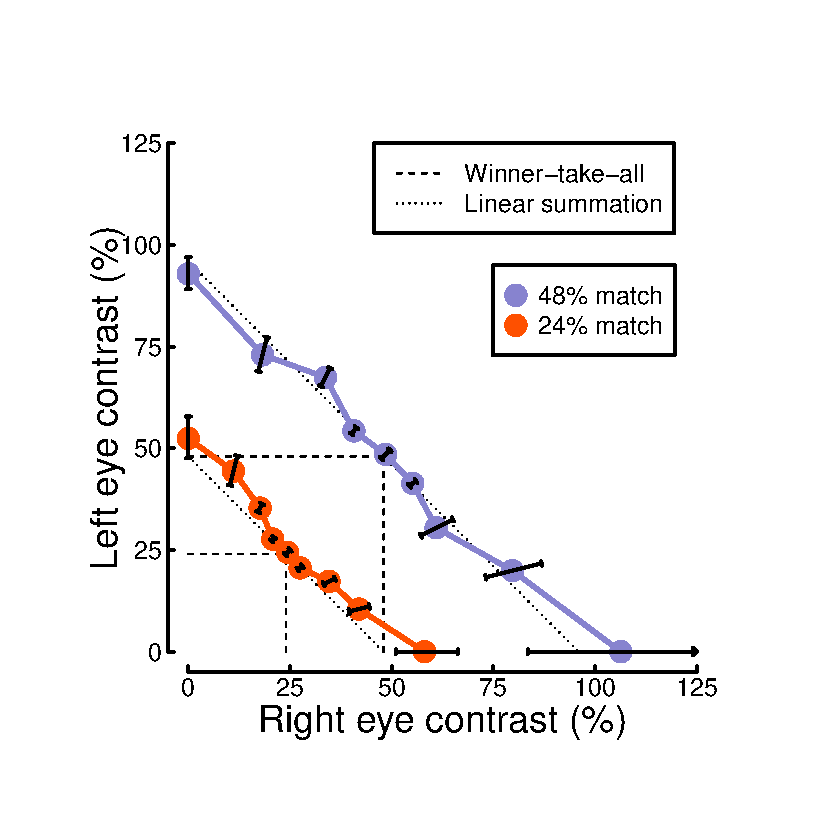
\includegraphics{Figures/matchingdata} 

}

\caption{Contrast matching functions. Dotted and dashed lines are predictions of canonical summation models with a linear exponent (dotted) or an infinite exponent (dashed). Error bars indicate the standard error across participants (N=10), and are constrained along radial lines converging at the origin. Interocular ratio distribution (from left to right of the figure): 1L0R, 1L0.25R, 1L0.5R, 1L0.75R, 1L1R, 0.75L1R, 0.5L1R, 0.25L1R, 0L1R.}\label{fig:matchingdata}
\end{figure}

\hypertarget{computational-modelling}{%
\subsection{Computational modelling}\label{computational-modelling}}

Several models have been developed and proposed to describe binocular combination and contrast matching results for spatial contrast. Among these, the models proposed by Ding and Sperling (2006) and Meese and colleagues (2006) are widely accepted. These models incorporate a dynamic contrast gain control, which allows to develop a model that combines binocular summation and interocular suppression

The first model is a multistage model that consists of two pairs of gain control mechanisms that inhibit each other (Ding and Sperling, 2006). In the earlier stage, the right and left eye channels exert gain control on the other channel. Then, they exert gain control on the other channel's gain control. Lastly, the outputs from each channel are summed binocularly to determine the binocular signal's magnitude.

The second model is similar as it also incorporates gain control mechanisms (Meese et al., 2006). In the first stage, it is applied to the left and right eye channels with suppression from the other eye. Then the signal from the two eyes is summed binocularly and gain control is applied a second time. This second model in particular is interesting and relevant as it was designed to also explain data from matching experiments.

We therefore decided to use and readapt this second model to see if it could be used to explain our three different data sets from experiments 1 and 3. In the first stage, the responses from the right and the left eyes are computed separately, as shown by equation 1 and 2:

\emph{RespL} = \(\frac{(L^q)}{Z + R + w \times R}\) (1)

\emph{RespR} = \(\frac{(R^q)}{Z + R + w \times L}\) (2)

where \emph{L} and \emph{R} are the signals from the left and right eyes, \emph{Z} is a saturation constant, \emph{q} is an exponent and \emph{w} is the suppression from the opponent weight.

In the second stage, the responses from the two eyes are summed binocularly:

\emph{Resp(L,R)} = k \(\times\) (RespL + RespR) + n

where \emph{k} is the noise parameter.

For our analysis, we implemented the model using a Bayesian approach, using the Stan software in Rstudio, which allowed us to generate a posterior parameter distribution. Results for this are shown in figure \ref{fig:modelfigure}i and the summary of the median parameter values are displayed in table \ref{tab:paramtable}. The key finding is that the pupillometry results display a much higher suppression from the opponent eye, shown by the \emph{w} parameter in table \ref{tab:paramtable} and the green line in figure \ref{fig:modelfigure}i, than the EEG results at the first harmonic (grey line in figure \ref{fig:modelfigure}i), the EEG results at the second harmonic (purple line in figure \ref{fig:modelfigure}i) and the matching results (yellow line in figure \ref{fig:modelfigure}i). These results offer an explanation to the data from the previous experiments: the higher suppression displayed by the pupillometry explains the non-linearity observed in the first experiment, while the lower suppression by the EEG at both harmonics and the matching explains the strong linearity observed in experiments 1 and 3.

Finally, figures \ref{fig:modelfigure}a-d show the behavioural data for our four main data sets from experiments 1 and 3, and figures \ref{fig:modelfigure}e-h show the outputs that the model produced based on the median parameter values that are presented in table \ref{tab:paramtable}. We can see that the data outputted by the model has a similar has a similar behaviour to the empirical data that we collected in our experiments. This would seem to suggest that the model can offer a good explanation of our data.

\begin{figure}

{\centering 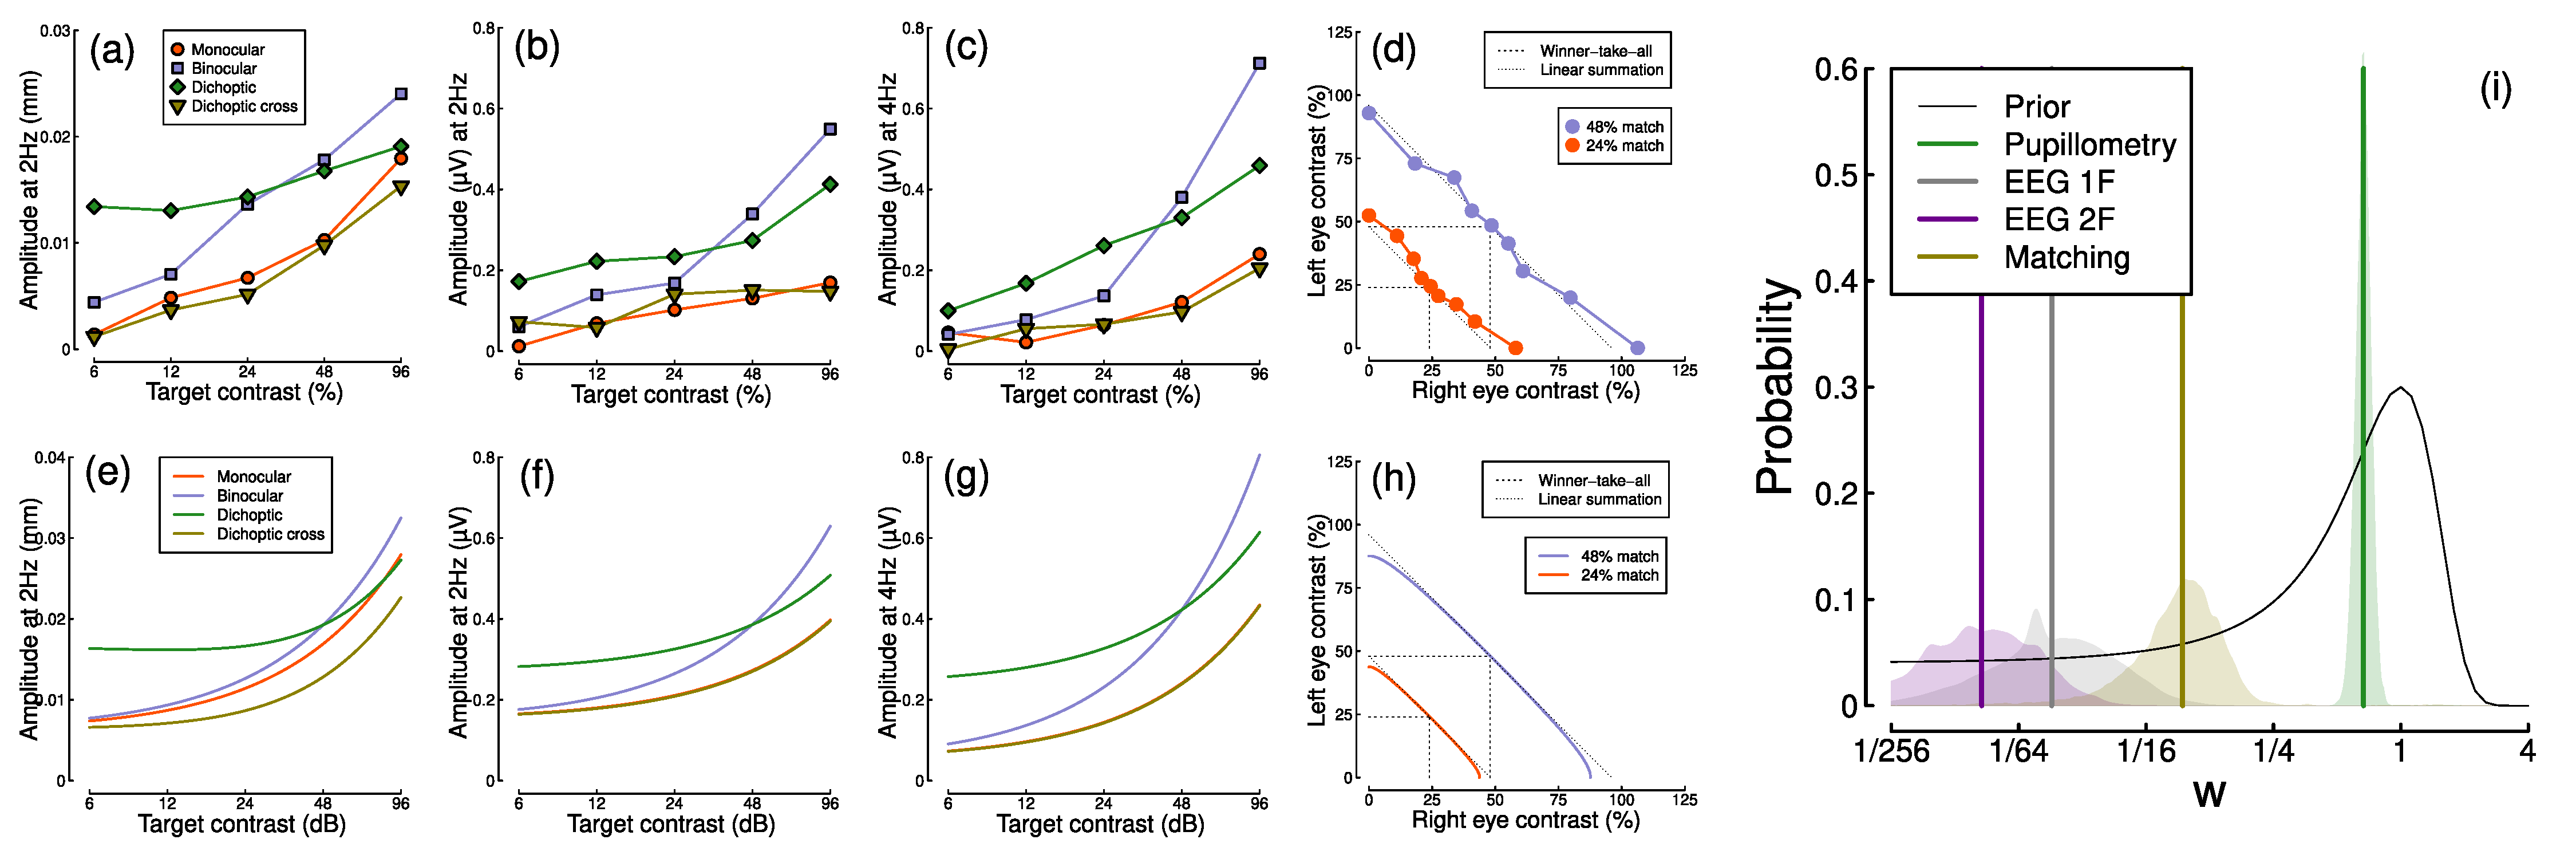
\includegraphics{Figures/modelfigure} 

}

\caption{Summary of computational modelling. Panels (a-d) show model behaviour for our four main data set, pupillometry (a), first harmonic EEG responses (b), second harmonic EEG responses (c) and contrast matching (d). Panel (i) shows the posterior probability distributions of the interocular suppression parameter for each of the four model fits. The pupillometry distribution (green) is centred about a substantially higher suppressive weight than for the other data types (note the logarithmic x-axis). The black curve shows the (scaled) prior distribution for the weight parameter.}\label{fig:modelfigure}
\end{figure}

\begin{table}

\caption{\label{tab:paramtable}Summary of median parameter values.}
\centering
\begin{tabular}[t]{l|c|c|c|c}
\hline
Data set & Z & k & w & Rmax\\
\hline
Pupillometry & 2.45 & 0.01 & 0.67 & 0.00024\\
\hline
EEG 1F & 2.78 & 0.15 & 0.03 & 0.00262\\
\hline
EEG 2F & 2.31 & 0.06 & 0.01 & 0.00407\\
\hline
Matching & 0.56 & 7.96 & 0.05 & -\\
\hline
\end{tabular}
\end{table}

\hypertarget{discussion}{%
\section{Discussion}\label{discussion}}

\hypertarget{references}{%
\section*{References}\label{references}}
\addcontentsline{toc}{section}{References}

\hypertarget{refs}{}
\begin{CSLReferences}{1}{0}
\leavevmode\vadjust pre{\hypertarget{ref-Anderson1989}{}}%
Anderson PA, Movshon JA. 1989. Binocular combination of contrast signals. \emph{Vision Res} \textbf{29}:1115--32. doi:\href{https://doi.org/10.1016/0042-6989(89)90060-6}{10.1016/0042-6989(89)90060-6}

\leavevmode\vadjust pre{\hypertarget{ref-Angee2021}{}}%
Angée C, Nedelec B, Erjavec E, Rozet J-M, Fares Taie L. 2021. Congenital microcoria: Clinical features and molecular genetics. \emph{Genes (Basel)} \textbf{12}. doi:\href{https://doi.org/10.3390/genes12050624}{10.3390/genes12050624}

\leavevmode\vadjust pre{\hypertarget{ref-Anstis1998}{}}%
Anstis S, Ho A. 1998. Nonlinear combination of luminance excursions during flicker, simultaneous contrast, afterimages and binocular fusion. \emph{Vision Res} \textbf{38}:523--39. doi:\href{https://doi.org/10.1016/s0042-6989(97)00167-3}{10.1016/s0042-6989(97)00167-3}

\leavevmode\vadjust pre{\hypertarget{ref-Baker2018}{}}%
Baker DH, Lygo FA, Meese TS, Georgeson MA. 2018. Binocular summation revisited: Beyond \(\sqrt{2}\). \emph{Psychol Bull} \textbf{144}:1186--1199. doi:\href{https://doi.org/10.1037/bul0000163}{10.1037/bul0000163}

\leavevmode\vadjust pre{\hypertarget{ref-Campbell1965}{}}%
Campbell FW, Green DG. 1965. Monocular versus binocular visual acuity. \emph{Nature} \textbf{208}:191--2. doi:\href{https://doi.org/10.1038/208191a0}{10.1038/208191a0}

\leavevmode\vadjust pre{\hypertarget{ref-Delorme2004}{}}%
Delorme A, Makeig S. 2004. EEGLAB: An open source toolbox for analysis of single-trial EEG dynamics including independent component analysis. \emph{J Neurosci Methods} \textbf{134}:9--21. doi:\href{https://doi.org/10.1016/j.jneumeth.2003.10.009}{10.1016/j.jneumeth.2003.10.009}

\leavevmode\vadjust pre{\hypertarget{ref-Ding2006}{}}%
Ding J, Sperling G. 2006. A gain-control theory of binocular combination. \emph{Proc Natl Acad Sci U S A} \textbf{103}:1141--6. doi:\href{https://doi.org/10.1073/pnas.0509629103}{10.1073/pnas.0509629103}

\leavevmode\vadjust pre{\hypertarget{ref-Kassner2014}{}}%
Kassner M, Patera W, Bulling A. 2014. Pupil: An open source platform for pervasive eye tracking and mobile gaze-based interactionProceedings of the 2014 {ACM} International Joint Conference on Pervasive and Ubiquitous Computing: Adjunct Publication. UbiComp '14 Adjunct; {ACM}. pp. 1151--1160. doi:\href{https://doi.org/10.1145/2638728.2641695}{10.1145/2638728.2641695}

\leavevmode\vadjust pre{\hypertarget{ref-Legge1984}{}}%
Legge GE. 1984. Binocular contrast summation--II. Quadratic summation. \emph{Vision Res} \textbf{24}:385--94. doi:\href{https://doi.org/10.1016/0042-6989(84)90064-6}{10.1016/0042-6989(84)90064-6}

\leavevmode\vadjust pre{\hypertarget{ref-Levelt1965}{}}%
Levelt WJ. 1965. BINOCULAR BRIGHTNESS AVERAGING AND CONTOUR INFORMATION. \emph{Br J Psychol} \textbf{56}:1--13. doi:\href{https://doi.org/10.1111/j.2044-8295.1965.tb00939.x}{10.1111/j.2044-8295.1965.tb00939.x}

\leavevmode\vadjust pre{\hypertarget{ref-Mathot2018}{}}%
Mathôt S. 2018. Pupillometry: Psychology, physiology, and function. \emph{J Cogn} \textbf{1}:16. doi:\href{https://doi.org/10.5334/joc.18}{10.5334/joc.18}

\leavevmode\vadjust pre{\hypertarget{ref-McDougal2010}{}}%
McDougal DH, Gamlin PD. 2010. The influence of intrinsically-photosensitive retinal ganglion cells on the spectral sensitivity and response dynamics of the human pupillary light reflex. \emph{Vision Res} \textbf{50}:72--87. doi:\href{https://doi.org/10.1016/j.visres.2009.10.012}{10.1016/j.visres.2009.10.012}

\leavevmode\vadjust pre{\hypertarget{ref-Meese2006}{}}%
Meese TS, Georgeson MA, Baker DH. 2006. Binocular contrast vision at and above threshold. \emph{J Vis} \textbf{6}:1224--43. doi:\href{https://doi.org/10.1167/6.11.7}{10.1167/6.11.7}

\leavevmode\vadjust pre{\hypertarget{ref-Purves2008}{}}%
Purves D, Brannon EM, Cabeza R, LaBar KS, Huettel SA, Platt ML, Woldorff MG. 2008. Principles of {Cognitive} {Neuroscience}. Oxford University Press, Incorporated.

\leavevmode\vadjust pre{\hypertarget{ref-Wang2015}{}}%
Wang C-A, Munoz DP. 2015. A circuit for pupil orienting responses: Implications for cognitive modulation of pupil size. \emph{Curr Opin Neurobiol} \textbf{33}:134--40. doi:\href{https://doi.org/10.1016/j.conb.2015.03.018}{10.1016/j.conb.2015.03.018}

\leavevmode\vadjust pre{\hypertarget{ref-Wyatt1981}{}}%
Wyatt HJ, Musselman JF. 1981. Pupillary light reflex in humans: Evidence for an unbalanced pathway from nasal retina, and for signal cancellation in brainstem. \emph{Vision Res} \textbf{21}:513--25. doi:\href{https://doi.org/10.1016/0042-6989(81)90097-3}{10.1016/0042-6989(81)90097-3}

\end{CSLReferences}

\end{document}
